\icode[magenta]{N13J-CO-CA-L4-260930-001}
\nceeID[20]{2013北京}{12}
对于同一物理问题，常常可以从宏观与微观两个不同角度进行研究，找出其内在联系，从而更加深刻地理解其物理本质。
\begin{enumerate}
	\item[(1)] 一段横截面积为\(S\)、长为\(l\)的直导线，单位体积内有\(n\)个自由电子，电子电量为\(e\)。该导线通有电流时，假设自由电子定向移动的速率均为\(v\)。
	\begin{enumerate}
		\item[(a)] 求导线中的电流\(I\)；
		\item[(b)] 将该导线放在匀强磁场中，电流方向垂直于磁感应强度\(B\)，导线所受安培力大小为\(F_\text{安}\)，导线内自由电子所受洛伦兹力大小的总和为\(F\)，推导\(F_\text{安}=F\)。
	\end{enumerate}
	\item[(2)] 正方体密闭容器中有大量运动粒子，每个粒子质量为\(m\)，单位体积内粒子数量\(n\)为恒量。为简化问题，我们假定：粒子大小可以忽略；其速率均为\(v\)，且与器壁各面碰撞的机会均等；与器壁碰撞前后瞬间，粒子速度方向都与器壁垂直，且速率不变。利用所学力学知识，导出器壁单位面积所受粒子压力\(f\)与\(m\)、\(n\)和\(v\)的关系。（注意：解题过程中需要用到、但题目没有给出的物理量，要在解题时做必要的说明）
\end{enumerate}	
\begin{answer}

	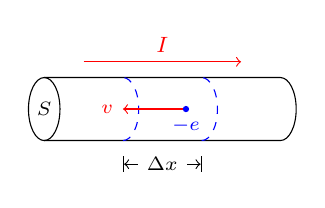
\begin{tikzpicture}
		\draw (0,0) ellipse(.2 and .4);
		\draw (0,-.4)--(3,-.4) arc(-90:90:.2 and .4)--(0,.4);
		\draw[blue,dashed] (1,-.4) arc(-90:90:.2 and .4) (2,-.4) arc(-90:90:.2 and .4);
		\draw[->,red] (1.8,0)--(1,0)node[left]{\scriptsize \(v\)};
		\fill[blue] (1.8,0)node[below]{\scriptsize \( - e\)} circle(.04);
		\draw[->,red] (.5,.6)--node[above]{\footnotesize \(I\)}(2.5,.6);
		\draw[|<->|] (1,-.7)--node[fill=white]{\scriptsize \(\Delta x\)}(2,-.7);
		\node at(0,0){\scriptsize \(S\)};
	\end{tikzpicture}
	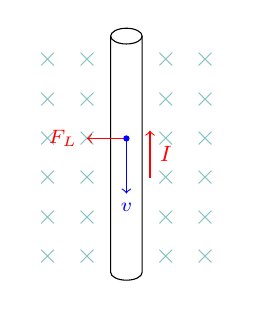
\begin{tikzpicture}
		\foreach \x in {-1,-.5,...,1}
			\foreach \y in {.2,.7,...,3}
				\node[teal!50] at(\x,\y){\( \times \)};
		\draw[fill=white] (-.2,3)--(-.2,0) arc(-180:0:.2 and .1)--(.2,3);
		\draw (0,3) ellipse(.2 and .1);
		\draw[->,red] (.3,1.2)--node[right]{\footnotesize \(I\)}(.3,1.8);
		\draw[->,blue] (0,1.7)--(0,1)node[below]{\scriptsize \(v\)};
		\draw[->,red] (0,1.7)--(-.5,1.7)node[left]{\scriptsize \(F_L\)};
		\fill[blue] (0,1.7) circle(.04);
	\end{tikzpicture}
	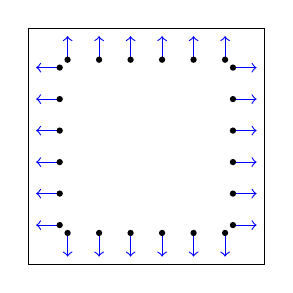
\begin{tikzpicture}
		\draw (0,0) rectangle(3,3);
		\foreach \x in {.5,.9,...,2.5}{
			\draw[->,blue] (\x,2.6)--++(0,.3);
			\fill (\x,2.6) circle(.04);
			\draw[->,blue] (\x,.4)--++(0,-.3);
			\fill (\x,.4) circle(.04);
			\draw[->,blue] (.4,\x)--++(-.3,0);
			\fill (.4,\x) circle(.04);
			\draw[->,blue] (2.6,\x)--++(.3,0);
			\fill (2.6,\x) circle(.04);}
	\end{tikzpicture}

	（1）(a)
	\begin{align*}
		Q&= N\cdot e = nV\cdot e = n\cdot \Delta xS\cdot e = n\cdot v\Delta t S\cdot e\\
		I&= \frac{Q}{\Delta t} = neSv
	\end{align*}
	
	(b)\begin{align*}
		F_L&= evB = e\cdot\frac{I}{neS}\cdot B = \frac{IB}{nS}\\
		F &= N\cdot F_L = nSL\cdot \frac{IB}{nS} = BIL = F_{\text{安}}
	\end{align*}
	
	（2）
	\begin{align*}
		\Delta p_0&= 2mv\\
		\Delta p&= N\cdot\Delta p_0 = \frac{1}{6}nV\cdot\Delta p_0 = \frac{1}{6}n\cdot v\Delta tS\cdot\Delta p_0\\
		F&=\frac{\Delta p}{\Delta t} = \frac{1}{6}nvS\cdot 2mv\\
		f&= \frac{F}{S} = \frac{1}{3}nmv^2 = \frac{2}{3}n\cdot E_k
	\end{align*}
\end{answer}